\documentclass[a4paper, 12pt]{report}
\usepackage[french]{babel}
\usepackage[utf8]{inputenc}
\usepackage[T1]{fontenc}
\usepackage{amsmath}
\usepackage{tabto}
\usepackage{graphicx}
\usepackage{titlesec}
\usepackage{hyperref}
\hypersetup{
  colorlinks=true,
  linktoc=none,
}

\titleformat{\chapter}[display]
  {\normalfont\bfseries}{}{0pt}{\Huge}

\titleformat{\section}[display]
  {\normalfont\bfseries}{}{0pt}{\Large}

\begin{document}

\begin{titlepage}

\centering


\includegraphics[width=0.45\textwidth]{images/gustave-eiffel-university.png}\par\vspace{1cm}

{\scshape\Large Projet de mathématiques appliquées\par}

\vspace{1.5cm}

{\huge\bfseries 2048\par}

\vspace{2cm}

{\Large\itshape Cloé \textsc{Quirin} \& Vincent \textsc{Scavinner}\par}

\vfill
supervisé par\par
Miguel \textsc{Martinez}
\vfill

{\large \today\par}

\end{titlepage}

\begin{abstract}
Rapport de projet documentant la réflexion et les choix d'implémentation réalisés dans le cadre de la conception d'une version revisitée du jeu 2048, utilisant des lois de probabilités mathématiques. 
Le code source du projet est disponible à l'adresse suivante : \href{https://github.com/vscav/2048}{https://github.com/vscav/2048}.
\end{abstract}

\tableofcontents

\chapter{Introduction}

\tabto{1cm}Cela fait maintenant quelques années que le jeu du 2048 a pris d'assaut Internet.
Dans le monde entier, des milliers de personnes ont passé des millions d'heures à
essayer de créer la tuile 2048.

\vspace{0.5cm}

\tabto{1cm}Outre le côté addictif du jeu, il présente également une possibilité
d'explorer les mathématiques. Dans le cadre d'un projet réalisé au cours d'une seconde année d'ingénieur
à l'IMAC (Univeristé Gustave Eiffel, Champs-sur-Marne, France), ce document tente de
démontrer la manière dont les théories et lois de probabilités ont été appliquées au jeu
original pour l'étendre et le renouveler dans une version revisitée.

\section{Règles}

\tabto{1cm}Le 2048 est un jeu \textit{"puzzle block"} développé par Gabriele Cirulli. C'est un jeu joué sur
une grille 4x4 avec des tuiles numérotées ${2^{n}}$ où ${n}$ représente un nombre naturel. L'objectif
du jeu est de combiner des tuiles du même nombre pour finalement former le nombre 2048.

\begin{figure}[!t]
\centering
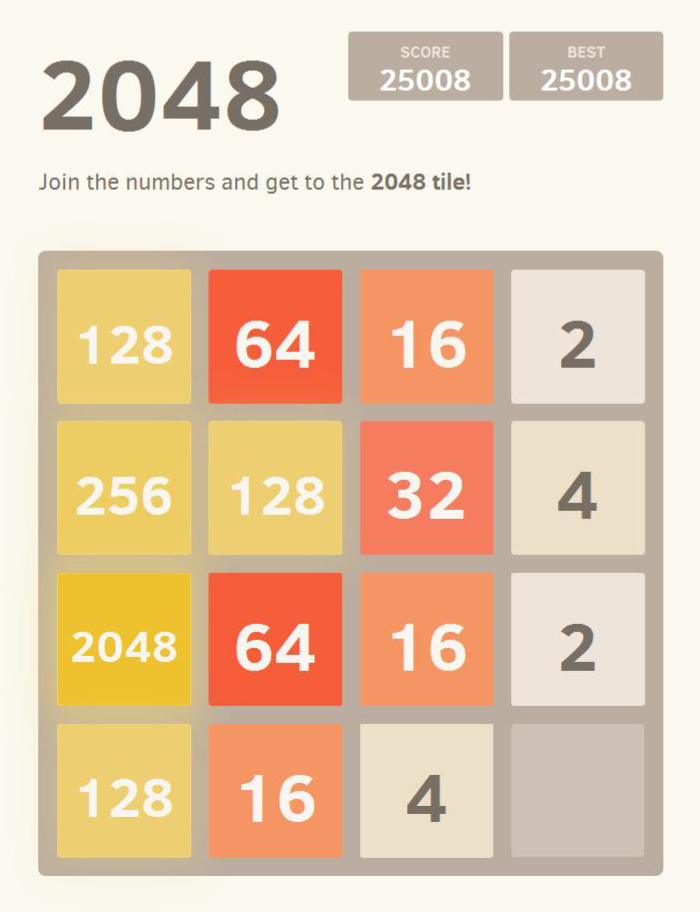
\includegraphics[width=0.55\textwidth]{images/2048-classic-version.jpg}
\caption{L'interface de la version classique}
\label{Classic version}
\end{figure}

\vspace{0.5cm}

\tabto{1cm}L'utilisateur peut se déplacer dans les quatre directions cardinales et après chaque mouvement,
une nouvelle tuile est générée (numérotée 2 ou 4) aléatoirement dans la grille. Un mouvement est
considéré comme "légal" si au moins une tuile peut être glissée dans un emplacement vide ou si les tuiles
peuvent être combinés dans la direction choisie. Le jeu se termine lorsque l'utilisateur n'a pas de mouvement
"légal" à gauche.

\section{Aspect mathématique de la version classique}

\tabto{1cm}Après avoir fait un mouvement, une nouvelle tuile est placée sur le plateau.
Celle-ci est placée aléatoirement sur un emplacement vide de la grille. Cette nouvelle tuile
peut avoir pour valeur un 2 ou un 4, là encore choisi aléatoirement. La valeur 2 a 90\% de chance
de tomber, tandis que la valeur 4 en a seulement 10. Le jeu continue ensuite jusqu'à ce qu'il n'y
ait plus de mouvements possibles.

\vspace{0.5cm}

\tabto{1cm}Outre cet aspect probabiliste, le coeur du jeu et de son intéractivité repose sur une
combinaison de transformations matricielles relative à la grille. Néanmoins, il est possible de
procéder à l'ensemble des mouvements nécessaires par un enchaînement de rotations matricielles.
C'est ce que nous avons choisi de faire dans le cadre de notre implémentation.

\chapter{Réinterprétation de l'original}

\tabto{1cm}Notre revisite du jeu classique se base essentiellement sur l'intégration de nouveaux types de tuiles.
\tabto{1cm}Il y a bien évidemment la tuile classique, qui possède la valeur 2 ou 4, chacune ayant une chance indépendante d'apparaître.
Mais nous avons intégrer trois types de tuiles supplémentaires : la tuile obstacle, mystère et bonus.
\tabto{1cm}La tuile obstacle est associée à un nombre de mouvements. Elle ne peut en aucun cas être fusionnée avec une autre tuile et son but est donc 
de vous bloquer dans certains cas. Elle disparaîtra seulement lorsque vous aurez effectuer le nombre de mouvements requis.
\tabto{1cm}La tuile bonus peut se fusionner à n'importe quelle autre tuile présente sur le plateau (même un obstacle). Pour cela, elle s'adapte et adopte la valeur
de la tuile cible (2 dans le cas de la fusion avec un obstacle).
\tabto{1cm}La tuile mystère représente une tuile de valeur, 2, 4, 8 ou 16. Seulement, il est impossible de le déterminer car la valeur est cachée.
Il faut la jouer et espérer tomber sur une tuile à la valeur correspondante. Rassurez-vous, la valeur finie par se révéler après un certain nombre de mouvements.

\begin{figure}[!t]
\centering
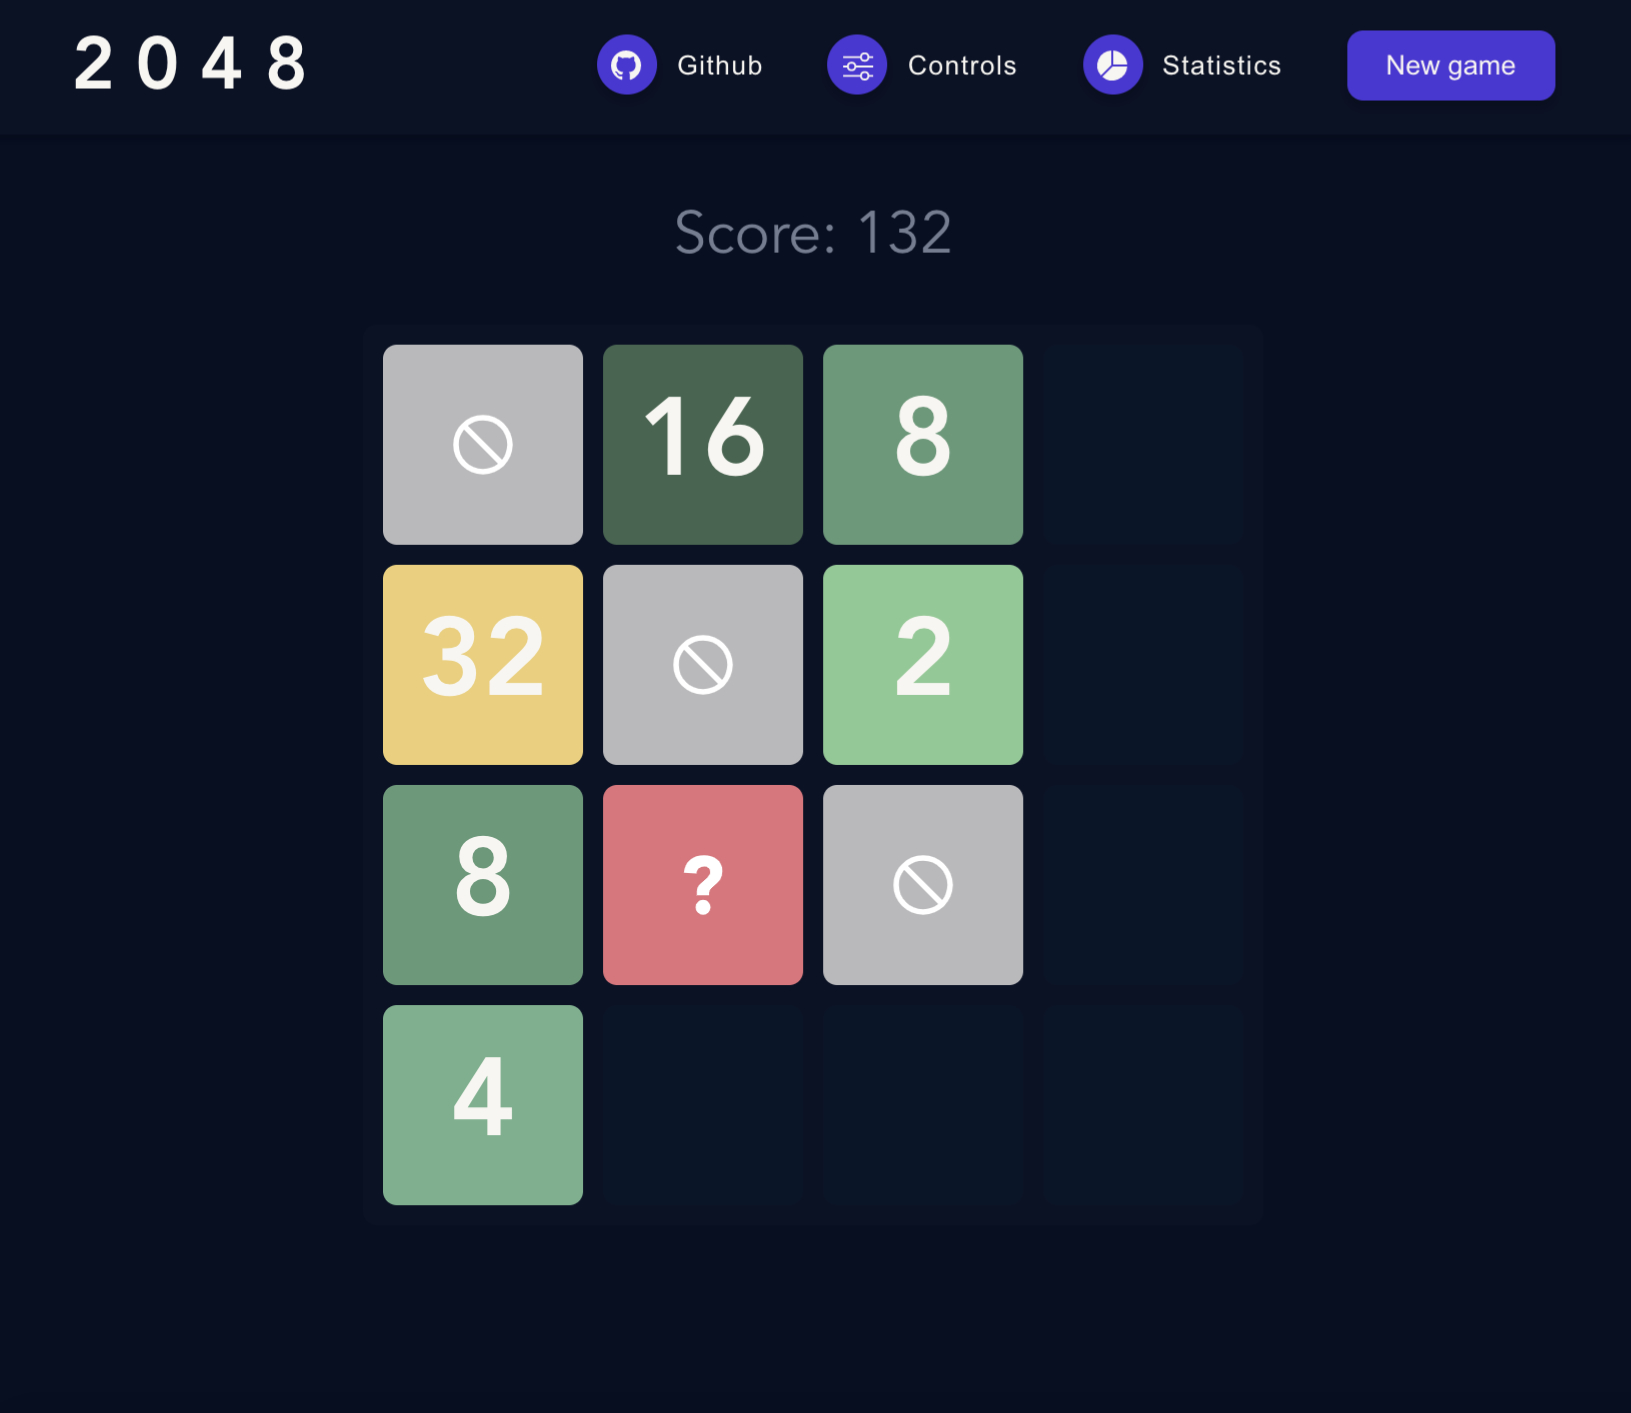
\includegraphics[width=1\textwidth]{images/2048-revisited-version.jpg}
\caption{L'interface de notre version du jeu}
\label{Revisited version}
\end{figure}

\vspace{0.5cm}

\tabto{1cm}.

\chapter{Les composantes aléatoires utilisées}

\begin{flushleft}

\section{Le type de tuile}

\textbf{Espace d'état :} Type de la nouvelle tuile.\break
\textbf{Loi choisie :} Loi géométrique.\break
\textbf{Pourquoi :} C’est une loi n’ayant que deux issues possibles.\break
\textbf{Paramètres :} Plus ou moins de chances de tomber sur des cellules spéciales qui peuvent aider ou bloquer le joueur.\break
\textbf{Comment :} On effectue un tirage aléatoire d’un nombre entre 0 et 1. Si cette valeur est inférieure à la valeur calculée par la loi géométrique, c’est un succès et la case est spéciale. 
Sinon, c’est un échec et la case est normale.\break

\begin{center}
${p(X=k)=(1-p)^{k-1}p}$
\end{center}

\section{Le type de la tuile spéciale}

\textbf{Espace d'état :} Type la tuile spéciale.\break
\textbf{Loi choisie :} Loi uniforme.\break
\textbf{Pourquoi :} Ici, on cherche seulement à savoir quel type de tuile spéciale va apparaître sur la grille. Tous les secteurs sont de même taille et ont la même probabilité.\break
\textbf{Paramètres :} Le jeu devient plus ou moins compliqué en fonction du type de case qui apparaît.\break
\textbf{Comment :} La variable aléatoire suit une loi uniforme sur l'intervalle [0,3]. On effectue un tirage aléatoire d’un nombre entre 0 et 1. En fonction du tirage, une des trois cases spéciales est sélectionnée.\break

\section{Valeur de la tuile classique}

\textbf{Espace d'état :} Valeur de la tuile classique.\break
\textbf{Loi choisie :} Loi de Bernoulli.\break
\textbf{Pourquoi :} La valeur de la cellule classique n’admet que 2 issues : 2 ou 4. Si on tombe sur 2, c’est un succès. Si on tombe sur 4, c’est un échec.\break
\textbf{Paramètres :} Plus ou moins de chances de tomber sur des cellules de valeur 4, rendant le jeu plus ou moins simple pour le joueur.\break
\textbf{Comment :} On effectue un tirage aléatoire d’un nombre entre 0 et 1.  Si ce nombre est inférieur au paramètre p, c’est un succès et la nouvelle case à pour valeur 2. 
Sinon, c’est un échec est la nouvelle case à pour valeur 4.\break

\begin{center}
${P(X = 1) = p, P(X = 0) = 1-p}$
\end{center}


\section{Tuile obstacle}

\textbf{Espace d'état :} Nombre de mouvements avant que la tuile obstacle ne disparaisse.\break
\textbf{Loi choisie :} Loi de Poisson.\break
\textbf{Pourquoi :} Ici, on veut compter le nombre d'événements en ne connaissant que le nombre moyen de ceux-ci.\break
\textbf{Paramètres :} Plus ou moins de chance que la case obstacle reste longtemps sur la grille.\break
\textbf{Comment :} k correspond au nombre de mouvement que le joueur doit effectuer avant que la case ne disparaisse et un paramètre modifiable par le joueur correspond au nombre de mouvements moyen necéssaires. 
On effectue des tirages aléatoires d’un nombre entre 0 et 1.  On compte alors le nombre de tirages qu’il faut avant que le nombre tiré soit inférieur au calcul de la probabilité. Si c’est inférieur, c’est un succès et la case disparaît.\break

\begin{center}
${p(X=k)=e^{-\lambda}\frac{\lambda^k}{k!}}$
\end{center}

\section{Tuile mystère}

\textbf{Espace d'état :} Nombre de mouvements avant que la tuile mystère ne soit révélée.\break
\textbf{Loi choisie :} Loi binomial.\break
\textbf{Pourquoi :} On réitère n fois un tirage de Bernoulli de manière indépendante.\break
\textbf{Paramètres :} Plus ou moins de chances que la case mystère soit révélé.\break
\textbf{Comment :} n, un paramètre modifiable par le joueur,  correspond au nombre de tirages et on fixe k à 1 car on souhaite obtenir un succès.\break

\begin{center}
${P(X=k)={n \choose k} p^k(1-p)^{n-k}}$
\end{center}

\end{flushleft}

\vspace{0.5cm}

\tabto{1cm}Les paramètres modifiables par le joueur pour influer sur le jeu sont accessibles depuis un menu de l'interface ("\textit{Controls}").
Nous avons mis en place des \textit{sliders} qui permettent au joueur d'avoir un impact sur quatre paramètres liés à quatre distributions différentes.

\tabto{1cm}De plus, une fenêtre modale ("\textit{Statistics}") permet (même en cours de partie) d'observer certaines statistiques de la partie. Par exemple, 
l'utilisateur a accès à une visualisation des proportions de distributions de chaque type de case. Cette visualisation est mise 
à jour de manière instantanée à chaque modification de valeurs via les sliders. Et de plus, les types de tuiles jouées sont comptabilisés afin 
de pouvoir s'assurer que cela correspond bien aux probabilités promises.

\begin{figure}[!t]
\centering
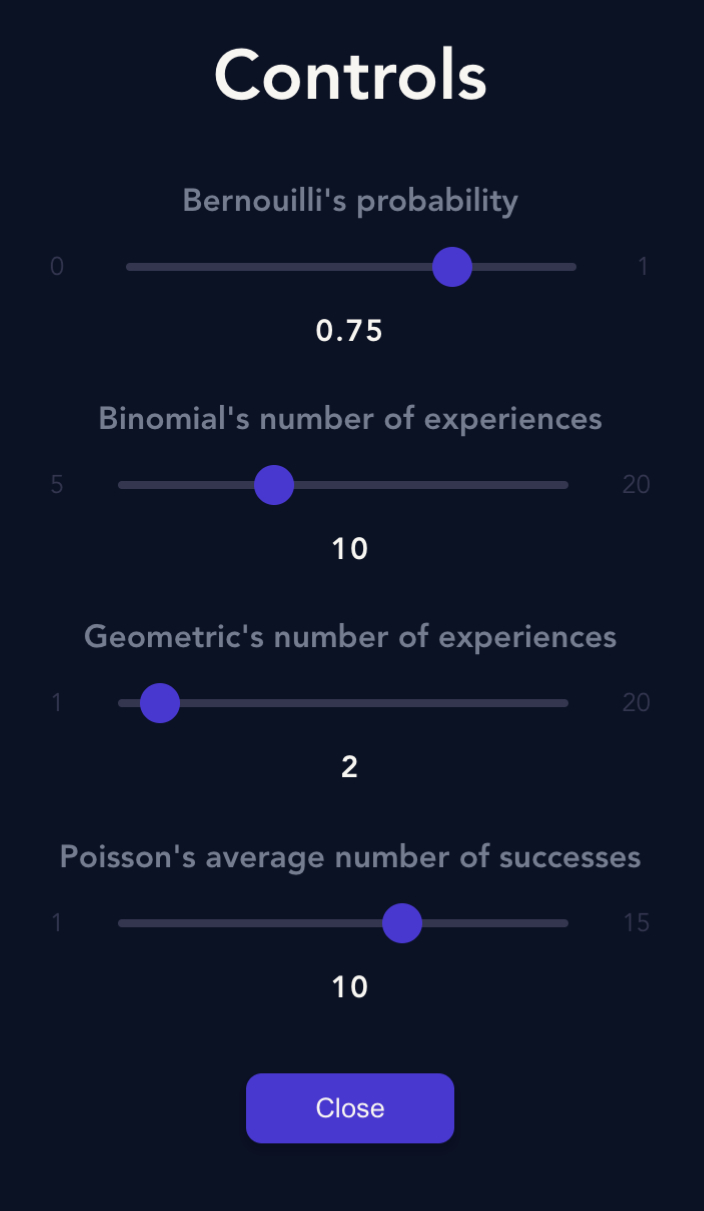
\includegraphics[width=0.4\textwidth]{images/2048-revisited-version-controls.jpg}
\caption{Control de certains paramètres via des sliders}
\label{Controls}
\end{figure}

\begin{figure}[!t]
\centering
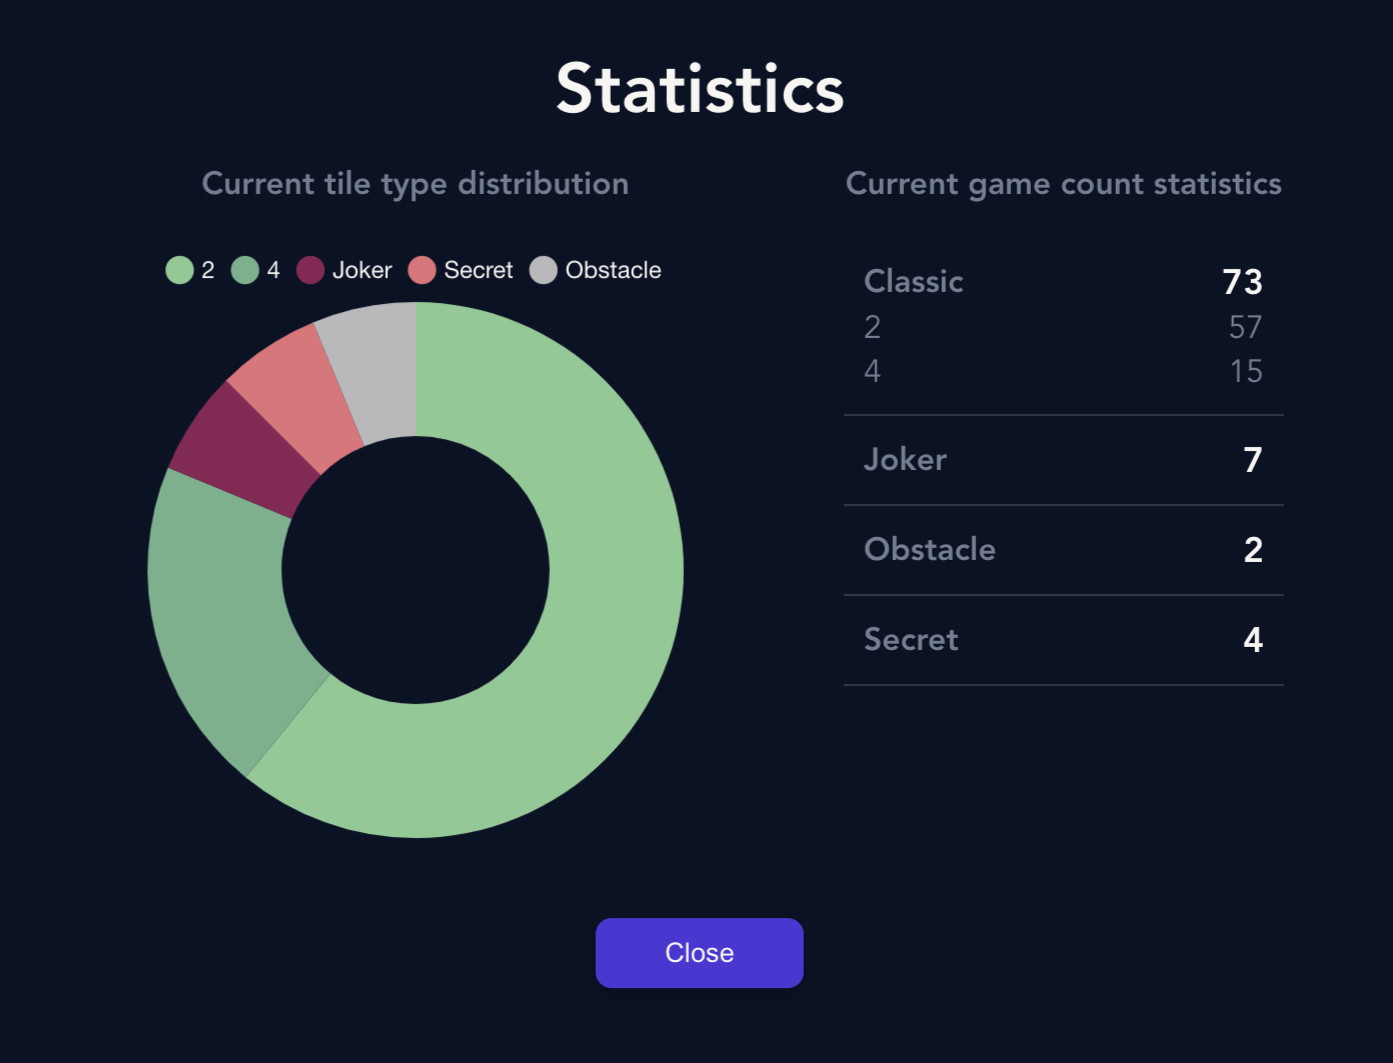
\includegraphics[width=0.5\textwidth]{images/2048-revisited-version-statistics.jpg}
\caption{Vérification de la cohérence via un panneau de statistiques}
\label{Statistics}
\end{figure}

\chapter{Technologies}

\section{Vue/TypeScript}

\tabto{1cm}Nous avons décidé d'utiliser le \textit{Framework Vue} mais dans une version typée grâce au
langage de programmation \textit{TypeScript}. Nous avons complété l'implémentation en utilisant du développement objet.

\vspace{0.5cm}

\tabto{1cm}\textit{Vue} (prononcé comme le terme anglais \textit{view}) est un \textit{framework} évolutif pour construire des
interfaces utilisateur. À la différence des autres \textit{frameworks} existants, \textit{Vue} a été conçu et pensé
pour pouvoir être adopté de manière incrémentale. Le cœur de la bibliothèque se concentre uniquement
sur la partie vue/\textit{front}, et il est vraiment simple de l’intégrer avec d’autres bibliothèques ou projets
existants.

\vspace{0.5cm}

\tabto{1cm}Contrairement à \textit{JavaScript}, le code écrit en \textit{TypeScript} est beaucoup plus fiable et facilement refactorable. 
Cela permet d'éviter les erreurs et de procéder à de la réécriture plus facilement.
La mise en place de types permet d'éviter des erreurs classiques et redondantes dans un code JavaScript classique,
et permet de se concentrer directement dessus afin d'éviter leur accumulation et le risque de bug majeur.
\tabto{1cm} \textit{TypeScript} permet également de s'intéresser plus en profondeur à la manière dont le système fonctionne vraiment.
Il permet de rendre abstrait des parties récurrentes afin de les réutiliser.
\tabto{1cm} Néanmoins, même si on peut facilement défendre l'idée d'utiliser \textit{TypeScript} dans un projet qui s'étend dans
le temps, il n'en est pas de même pour un projet à court terme comme le nôtre. En effet, typer correctement un projet
demande beaucoup de temps, beaucoup de minutie et beaucoup de réflexion.

\section{Librairies personnalisées}

\tabto{1cm}Nous avons fait le choix de créer notre propre librairie mathématique, chargée de nous fournir facilement les distributions et lois
dont nous avions besoin. Cela nous a permis de réaliser un couplage faible avec le reste de notre jeu, mais aussi de préparer
l'éventualité d'une évolution de l'application avec de nouvelles probabilités. Notre jeu possède donc son propre \textit{Manager}, chargé 
de faire les appels à notre librarie.

\vspace{0.5cm}

\tabto{1cm}En plus des probabilités, le jeu repose également sur des transformations
matricielles. Nous avons alors créé notre propre fonction utilitaire afin de réaliser ces transformations le plus
simplement possible. Cette fonction a été implémentée de manière générique grâce à TypeScript.

\vspace{0.5cm}

\tabto{1cm}Enfin, au cours d'une partie, les structures de données chargées de stocker les états relatifs aux différentes tuiles
(couramment en jeu ou celles déjà jouées) peuvent potentiellement atteindre des tailles importantes. Pour optimiser les recherches, 
nous avons décidé de réinterpréter la fonction de filtre (\textit{Array.filter()}) sur tableaux de \textit{JavaScript}.
Après quelques tests, notre implémentation s'avère en moyenne 60\% plus rapide. Nous en avons aussi profiter pour écrire une fonction
de filtre mais applicable à des objets. Pour cela, nous avons mis en place le principe de \textit{currying}.

\vspace{0.5cm}

\tabto{1cm}Nous avons mis en place des tests sur chacune des libraries pour vérifier la cohérence des résultats retournés par les fonctions.
Ces tests sont notamment primordiaux sur les retours des méthodes des lois de distribution. Ainsi nous avons pu mettre en place des tests pour
vérifier que les résultats retournés par nos lois uniformes, nos lois de Poisson et nos lois de Bernouilli étaient corrects. Pour cela, nous
vérifions que la valeur de retour est bien supérieure au minimum attendu et inférieure au maximum attendu, mais nous vérifions également que la 
médiane et la variance sont bien proches de celles attendues (avec un degré d'erreur calculé en fonction du nombre d'essais, fixés à 1 million pour les tests).

\chapter{Conclusion}

\tabto{1cm}Nous espérons avoir réussi à montrer que derrière un simple jeu, il y a un monde
mathématique à explorer. Les concepts étudiés ce semestre et les ressources consultées au
cours du projet nous ont aidé à analyser le jeu et son fonctionnement, mais aussi à l'aborder
sous des angles différents afin de comprendre comment y implanter des lois de probabilités
pour le rendre d'autant plus ludique. L'intéractivité offerte à l'utilisateur via un contrôle
sur certains paramètres lui permet de visualiser l'impact qu'ils ont au cours du jeu et l'oblige 
potentiellement à adopter de nouvelles stratégies pour résoudre le puzzle.

\end{document}